\subsection{Esercizio 6 pag.237   Hoff}

Poisson population comparisons: let’s reconsider the number of children data of Exercise 4.8. We’ll assume Poisson sampling models for the two
groups as before, but now we’ll parameterize $\theta_{A}$ and $\theta_B$ as $\theta_A$ = $\theta$, $\theta_B$ = $\theta_A \times \gamma$. In this parameterization, $\gamma$ represents the relative rate $\theta_B/\theta_A$. Let $\theta \sim$ Gamma $(a_\theta, b_\theta)$ and let $\gamma \sim$ Gamma$(a_\gamma, b_\gamma)$.
\begin{enumerate}
\item [a)]Are $\theta_A$ and $\theta_B$ independent or dependent under this prior distribution?
In what situations is such a joint prior distribution justified?
\item [b)]Obtain the form of the full conditional distribution of $\theta$ given $y_A$, $y_B$ and $\gamma$.
\item [c)]Obtain the form of the full conditional distribution of $\gamma$ given $y_A$, $y_B$ and $\theta$.
\item [d)]Set $a_\theta$ = 2 and $b_\theta$ = 1. Let $a_\gamma$ = $b_\gamma \in \lbrace 8, 16, 32, 64, 128 \rbrace $. For each of these five values, run a Gibbs sampler of at least 5,000 iterations and obtain E$[\theta_B - \theta_A|y_A, y_B]$. Describe the effects of the prior distribution for $\gamma$ on the results.
\end{enumerate}

\textbf{Svolgimento}:
\bigskip

A e B indicano due popolazioni di uomini di 30 anni con e senza laurea, rispettivamente, di cui vogliamo calcolare il numero medio di figli.\\

Sia Y il numero dei figli.\\

Per quanto riguarda la popolazione A, abbiamo $Y|\theta_A \sim$ Poisson$(\theta_A)$ con $\theta_A=\theta$.\\

Similmente, per la popolazione B abbiamo $Y|\theta_B \sim$ Poisson$(\theta_B)$ con $\theta_B=\theta \times \gamma$.\\ 

Dal momento che
\begin{itemize}
\item $\theta \sim$ Gamma$(a_\theta, b_\theta)$
\item $\gamma \sim$ Gamma$(a_\gamma, b_\gamma)$
\item $\theta \perp \gamma$
\end{itemize}

il modello delle osservazioni può essere riscritto come\\

$Y|\theta \sim$ Poisson$(\theta)$ per A\\

$Y|\theta, \gamma \sim$ Poisson$(\theta\gamma)$ per B.\\

Una volta ricavato $\theta$, e di conseguenza $\theta_A$, possiamo calcolare $\theta_B$ essendo uguale a $\theta \times \gamma$.
In particolare se:
\begin{itemize}
\item $\theta$ = 1, allora $\theta_A = \theta_B$
\item $\theta >$ 1, allora $\theta_A > \theta_B$
\item $\theta <$ 1, allora $\theta_A < \theta_B$
\end{itemize}

La riparametrizzazione $\theta_A$ = $\theta$, $\theta_B$ = $\theta \times \gamma$ è di conseguenza un'operazione utile per analizzare e confrontare le due distribuzioni.

\begin{enumerate}
\item [a)] Per poter valutare se $\theta_A$ e $\theta_B$ sono indipendenti, calcoliamo il valore della covarianza $Cov(\theta_A, \theta_B)$.\\

$Cov(\theta_A, \theta_B)$ = \\

= E$(\theta_A\theta_B)$ - E$(\theta_A)$E$(\theta_B)$ =\\

= E$(\theta^2\gamma)$ - E($\theta$)E$(\theta\gamma)$ =\\

= $\int_\theta \int_\gamma \theta^2 p(\theta,\gamma) d\theta d\gamma$ - E($\theta$)$\int_\theta \int_\gamma \theta p(\theta,\gamma) d\theta d\gamma$ =\\

= $\int_\theta \theta^2 p(\theta)d\theta \int_\gamma p(\gamma)d\gamma $ - E($\theta$)$\int_\theta \theta p(\theta)d\theta \int_\gamma \gamma p(\gamma)d\gamma$ = \\

= E$(\theta^2)$E($\gamma$) - E$(\theta)^2$E$(\gamma)$ = \\

= E$(\gamma)$(E$(\theta^2)$ - E$(\theta)^2)$ =\\

= E$(\gamma)Var(\theta)$\\

Tale quantità è maggiore di 0, quindi $\theta_A$ e $\theta_B$ sono linearmente dipendenti.

Si può verificare tale dipendenza anche con un ragionamento meno formale, considerando la seguente uguaglianza:\\

$p(\theta_B|\theta_A)=p(\theta\gamma|\theta)$\\

$\theta$ compare non solo nella variabile, ma anche nel "lato" della condizione.\\
Per tale ragione, $\theta_A$ e $\theta_B$ sono dipendenti.

Adesso consideriamo la distribuzione di Poisson per analizzare degli eventi relativi a un certo intervallo di tempo. Esaminiamo due casi distinti, A e B, ai quali sono associati $\theta_A$ e $\theta_B$ per misurare gli eventi che si verificano. In particolare, sappiamo che 
$\theta_A = \theta$ e che $\theta_B = \theta\gamma$.
Il numero degli eventi di B è influenzato $\gamma$: si tratta perciò di un parametro che differenzia B rispetto alle condizioni "standard" di A.\\
La distribuzione congiunta a priori può essere dunque utilizzata in situazioni analoghe a quella appena descritta, ossia quando abbiamo l'obiettivo di esaminare i cambiamenti su una determinata popolazione rispetto a un'altra di partenza. \\

\item [b)]
Per ricavare la distribuzione full conditional di $\theta$, come primo passo dobbiamo definire il Markov blanket, poi applicare la proprietà locale di Markov.
\\

\begin{center}
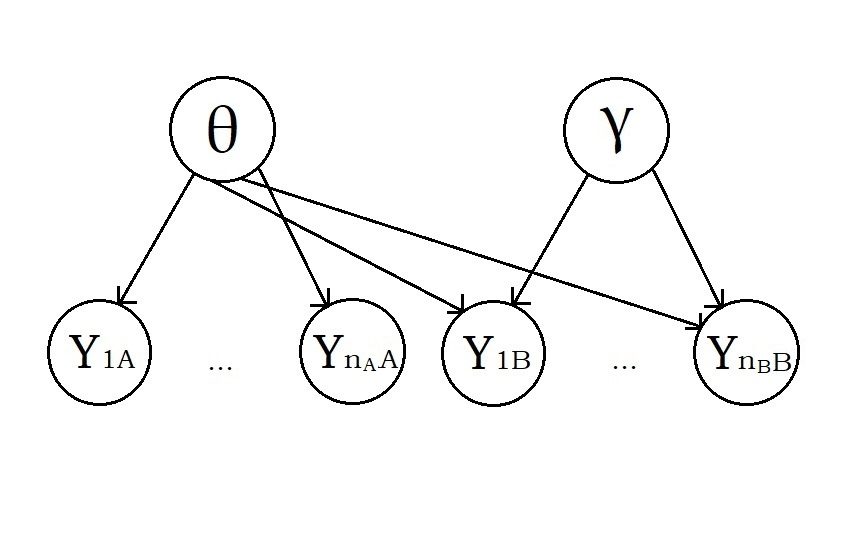
\includegraphics[scale=0.4]{img/esercizio6-01-grafo61.jpg}
\end{center}

Come si può osservare dallo schema, i figli di $\theta$ sono le osservazioni di A, quelle di B e $\gamma$ (questo perchè le osservazioni di B hanno come nodo padre anche $\gamma$). Inoltre $\theta$ non ha alcun nodo padre. \\
Quindi il Markov blanket risulta: \\
$bl(\theta)$ = $\lbrace Y_{1A}, Y_{2A} \ldots Y_{n_AA}, Y_{1B}, Y_{2B} \ldots Y_{n_BB}, \gamma\rbrace$.\\

Dunque\\
$p(\theta|y_{1A}, y_{2A} \ldots y_{n_AA}, y_{1B}, y_{2B} \ldots y_{n_BB}, \gamma) \propto$\\

$\propto p(\theta|a_\theta, b_\theta)$ $\prod_{i=1}^{n_A}{p(y_{iA}|\theta)} \prod_{j=1}^{n_B}{p(y_{jB}|\theta, \gamma)}$ =\\

$ = \frac{b_\theta^{a_\theta}}{\Gamma(a_\theta)}\theta^{a_\theta-1}e^{-b_\theta\theta} \prod_{i=1}^{n_A}{\frac{\theta^{y_{iA}} e^{-\theta}}{y_{iA}!}} \prod_{j=1}^{n_B}{\frac{(\theta\gamma)^{y_{jB}}e^{-\theta\gamma}}{y_{jB}!}}$ $\propto$\\

$\propto \theta^{a_\theta-1}e^{-b_\theta\theta}\theta^{\sum_{i=1}^{n_A}{y_{iA}}}e^{-n_A\theta}(\theta\gamma)^{\sum_{j=1}^{n_B}{y_{jB}}}e^{-n_B\theta\gamma}\simeq$\\

$\simeq \theta^{a_\theta + \sum_{i=1}^{n_A}{y_{iA}} + \sum_{j=1}^{n_B}{y_{jB}-1}}$ $ e^{-\theta(b_\theta+n_A+n_{B\gamma})}$

Da cui\\
$\theta|y_{1A},\ldots,y_{n_AA},y_{1B},\ldots,y_{n_BB}, \gamma \sim Gamma(a_\theta + \sum_{i=1}^{n_A}y_{iA} + \sum_{j=1}^{n_B}y_{jB}, b_\theta + n_A + n_{B}\gamma) $.\\


\item [c)]
Procediamo in modo simile al punto precedente, ricavando il Markov blanket di $\gamma$. \\ 
$\gamma$ non ha padre, e i suoi figli sono le osservazioni di B, che a loro volta hanno come genitore anche $\theta$ (come già detto). 
Dunque  il Markov blanket di $\gamma$ è $bl(\gamma)$ = $\lbrace  Y_{1B}, Y_{2B} \ldots Y_{n_BB}, \theta\rbrace$.\\


$p(\gamma|y_{1A}, y_{2A} \ldots y_{n_AA}, y_{1B}, y_{2B} \ldots y_{n_BB}, \theta) = $\\

$= p(\gamma|y_{1B}, y_{2B} \ldots y_{n_BB}, \theta) \propto $\\

$\propto p(\gamma|a_\gamma, b_\gamma)$ $\prod_{i=1}^{n_B}{p(y_{iB}|\theta,\gamma)} $ = \\

$= \frac{b_\gamma^{a_\gamma}}{\Gamma(a_\gamma)} \gamma^{a_\gamma-1}e^{-b_\gamma\gamma} \prod_{i=1}^{n_B}{\frac{(\theta\gamma)^{y_{iB}}e^{-\theta\gamma}}{y_{iB}!}} \propto $ \\

$\propto \gamma^{a_\gamma-1}e^{-b_\gamma\gamma}(\theta\gamma)^{\sum_{i=1}^{n_B}{y_{iB}}}e^{-n_B\theta_\gamma} \propto $ \\

$ \propto\gamma^{a_\gamma + \sum_{i=1}^{n_B}{y_{iB}-1} e^{-\gamma(b_\gamma+n_B\theta)}}$\\

Anche in questo caso possiamo riconoscere il kernel di una Gamma, perciò\\

$\gamma|y_{1A},\ldots,y_{n_AA},y_{1B},\ldots,y_{n_BB},\theta$ $\sim$ Gamma$(a_\gamma + \sum_{i=1}^{n_B}y_{iB} + b_\gamma + n_{B}\theta)$.\\

 
\item [d)] Riportiamo di seguito il codice R relativo all'algoritmo di Gibbs.

Come indicato nel testo dell'esercizio 4.8, i dataset utilizzati sono presenti nei file menchild30bach.dat
e menchild30nobach.dat.

Procediamo con l'inizializzazione dei dati:
\begin{verbatim}

>A<-c(1, 0, 0, 1, 2, 2, 1, 5, 2, 0, 0, 0, 0, 0,
+ 0, 1, 1, 1, 0, 0, 0, 1, 1, 2, 1, 3, 2, 0, 0,
+ 3, 0, 0, 0, 2, 1, 0, 2, 1, 0, 0, 1, 3, 0, 1,
+ 1, 0, 2, 0, 0, 2, 2, 1, 3, 0, 0, 0, 1, 1)

> B<-c(2, 2, 1, 1, 2, 2, 1, 2, 1, 0, 2, 1, 1, 2,
+ 0, 2, 2, 0, 2, 1, 0, 0, 3, 6, 1, 6, 4, 0, 3, 2, 0, 1,
+ 0, 0, 0, 3, 0, 0, 0, 0, 0, 1, 0, 4, 2, 1, 0, 0, 1, 0,
+ 3, 2, 5, 0, 1, 1, 2, 1, 2, 1, 2, 0, 0, 0, 2, 1,
+ 0, 2, 0, 2, 4, 1, 1, 1, 2, 0, 1, 1, 1, 1, 0, 2, 3, 2,
+ 0, 2, 1, 3, 1, 3, 2, 2, 3, 2, 0, 0, 0, 1, 0, 0,
+ 0, 1, 2, 0, 3, 3, 0, 1, 2, 2, 2, 0, 6, 0, 0, 0, 2, 0,
+ 1, 1, 1, 3, 3, 2, 1, 1, 0, 1, 0, 0, 2, 0, 2, 0,
+ 1, 0, 2, 0, 0, 2, 2, 4, 1, 2, 3, 2, 0, 0, 0, 1, 0, 0, 1,
+ 5, 2, 1, 3, 2, 0, 2, 1, 1, 3, 0, 5, 0, 0, 2,
+ 4, 3, 4, 0, 0, 0, 0, 0, 0, 2, 2, 0, 0, 2, 0, 0, 1, 1, 0,
+ 2, 1, 3, 3, 2, 2, 0, 0, 2, 3, 2, 4, 3, 3, 4,
+ 0, 3, 0, 1, 0, 1, 2, 3, 4, 1, 2, 6, 2, 1, 2, 2)

\end{verbatim}

Adesso effettuiamo l'inizializzazione dei parametri delle varie distribuzioni, poi settiamo il numero delle iterazioni da eseguire e il seed:

\begin{verbatim}
> a_theta<-2
> b_theta<-1
> v_gamma<-c(8, 16, 32, 64, 128)
> 
> n<-5000
> set.seed(150)
\end{verbatim}

Per la distribuzione gamma facciamo uso di un vettore perchè dobbiamo valutare i risultati per $a_\gamma$ = $b_\gamma \in \lbrace 8, 16, 32, 64, 128 \rbrace $.\\
Inizializziamo inoltre il vettore delle medie, il cui uso verrà chiarito a breve
\begin{verbatim}
> valori_medie<-NULL
\end{verbatim}

Nell'algoritmo di Gibbs viene eseguito un doppio ciclo: nel for più interno, per ognuna delle 5 coppie di iperparametri, vengono simulate le distribuzioni full conditionall (con 5000 valori sia per theta che per gamma); in ognuna delle iterazioni del for più esterno, vengono invece calcolati i valori attesi. \\ \\
Per comodità, facciamo uso di un array in 3 dimensioni: le prime due fanno riferimento a una matrice (5000 $\times$ 2) in cui vengono memorizzati i valori campionati di theta e gamma per ogni iterazione; la terza dimensione (5) serve per rieseguire questi passi, variando però gli iperparametri dell'a priori della distribuzione gamma.

\begin{verbatim}
> gibbs<-array(NA, c(n, 2, 5))
\end{verbatim}

Prima di eseguire l'algoritmo, calcoliamo, per ogni gruppo, le numerosità e i totali.
\begin{verbatim}
> nA<-length(A)
> nB<-length(B)
> 
> ytotA<-sum(A)
> ytotB<-sum(B)
> ytot<-ytotA+ytotB
\end{verbatim}

Tali valori caratterizzano i parametri delle full conditional.\\

Adesso inizializziamo i parametri gamma, theta e k: 
\begin{verbatim}
> gamma<-1
> theta<-1
> k<-1
\end{verbatim}

Come passo successivo, eseguiamo l'algoritmo:
\begin{verbatim}
> for(i in v_gamma){
+ a_gamma<-b_gamma<-i
+ for(j in 1:n){
+ theta<-rgamma(1, a_theta+ytot, b_theta+nA+nB*gamma)
+ gamma<-rgamma(1, a_gamma+ytotB, b_gamma+nB*theta)
+ gibbs[j,,k]<-cbind(theta, gamma)
+ }
+ k<-k+1
+   }
\end{verbatim}

Considerato che vogliamo ricavare il valore atteso della differenza tra thetaB e thetaA, dobbiamo calcolare la trasformazione theta*gamma-theta per ogni estrazione di theta e gamma ed eseguire la media su tutte le simulazioni. \\
Questo è possibile perchè abbiamo a disposizione il campione della congiunta a posteriori sia di theta che di gamma. \\
Ovviamente il procedimento deve essere ripetuto per ognuna delle 5 possibili scelte degli iperparametri della a priori di gamma, perciò memorizziamo i vari risultati nell'array valori\textunderscore medie.

\begin{verbatim} 
> for (i in 1:5){
+ valori_medie<-c(valori_medie, mean(gibbs[,1,i]*gibbs[,2,i]
+ -gibbs[,1,i]))
+  }
> valori_medie
[1] 0.3910311 0.3388716 0.2708131 0.2026279 0.1333113
\end{verbatim}

Come si può notare nell'output, il valore atteso della differenza tra thetaB e thetaA diminuisce 
progressivamente all'aumentare dei parametri dell'a priori di gamma. \\
Quindi, il numero di figli tra le due popolazioni prese in esame, decresce.

\begin{verbatim}
> leg<-v_gamma
> leg.txt<-rep("ab=bb",5)
> 
> par(mfrow=c(3,2))
> for(i in 1:5){
+ hist(gibbs[,1,i],prob=T,col="red",ylim=c(0,5),xlim=c(0,2.5),
+ ylab="densità a posteriori",xlab="numero medio di figli",main="")
+ lines(density(gibbs[,1,i]))
+ hist(gibbs[,1,i]*gibbs[,2,i],prob=T,col="blue",add=T)
+ lines(density(gibbs[,1,i]*gibbs[,2,i]))
+ }
> for(i in 1:5){
+ hist(gibbs[,1,i],prob=T,col="red",ylim=c(0,5),xlim=c(0,2.5),
+ ylab="densità a posteriori",xlab="numero medio di figli",main="")
+ lines(density(gibbs[,1,i]*gibbs[,2,i]))
+ hist(gibbs[,1,i]*gibbs[,2,i],prob=T,col="blue",add=T)
+ lines(density(gibbs[,1,i]*gibbs[,2,i]))
+ text(2, 4.5, paste("a_gamma=",lege[i]))
+ text(2, 3.5, paste("b_gamma=",lege[i]))
+ }
> 
\end{verbatim} 

\begin{center}
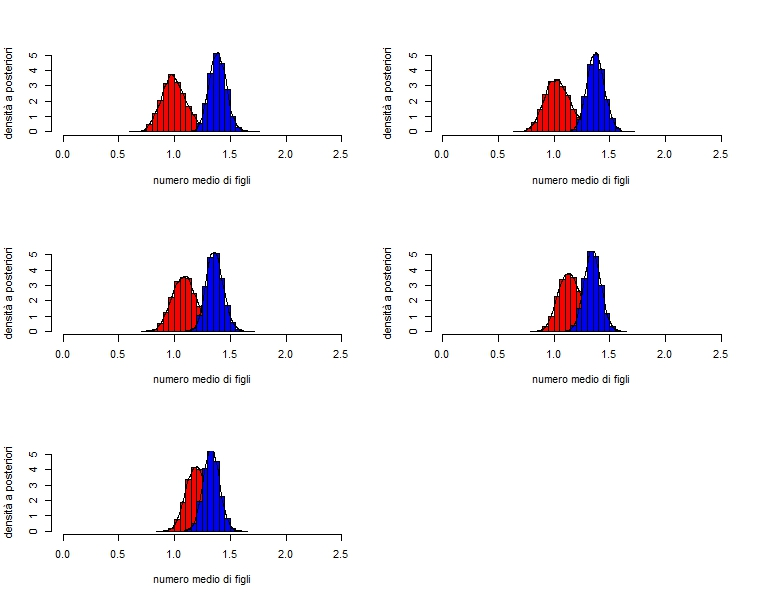
\includegraphics[scale=0.5]{img/esercizio6-01-grafo1.jpeg}
\end{center}

Quanto detto precedentemente, è evidente anche osservando i grafici.
La parte in rosso rappresenta thetaA, quella blu thetaB.
Come si può notare, le due distribuzioni sono sempre più vicine l'una all'altra all'aumentare degli iperparametri dell'a priori.

\begin{verbatim}
> x<-seq(0, 10, by=0.01)
> par(mfrow=c(1,1))
> plot(x, dgamma(x,8,8),type="l",xlim=c(0,5),ylim=c(0,5),
+ xlab=expression(gamma),ylab=expression(p(gamma)),
+ main="gamma a priori",col=1)


> for(j in 2:5){
+ curve(dgamma(x,v_gamma[j],v_gamma[j]),add=T,col=j)
+ }
> legend(2,4,c("a_gamma=b_gamma=8","a_gamma=b_gamma=16",
+ "a_gamma=b_gamma=32", "a_gamma=b_gamma=64",
+ "a_gamma=b_gamma=128"),col=c(1,2,3,4,5),lty=1)
\end{verbatim}

\begin{center}
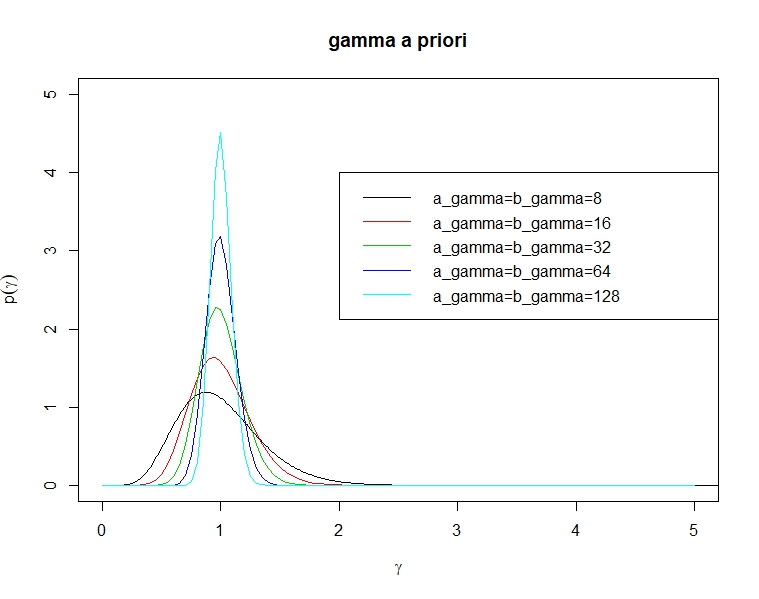
\includegraphics[scale=0.5]{img/esercizio6-01-grafo2.jpeg}
\end{center}

Osserviamo questo grafico: al crescere del numero degli iperparametri, l'apriori si "allunga" attorno a 1,
ossia il valore atteso.
Per quanto riguarda invece la varianza, questa risulta inversamente proporzionale al valore dei parametri.
Di conseguenza, la scelta degli iperparametri influisce molto sull'inferenza.
Più aumentano i valori di quest'ultimi, maggiore informazione è racchiusa nell'a priori: possiamo affermare ciò se consideriamo sia il cambiamento di tale distribuzione, sia il progressivo avvicinarsi di thetaA e thetaB.
Tenderemo quindi a ignorare thetaA e thetaB, e a fare affidamento solo sull'a priori.

\begin{verbatim}
> library(coda)
> effectiveSize(gibbs[,,1])

    var1     var2 
609.1041 605.4248 
\end{verbatim}

Con quest'ultime istruzioni, attraverso le quali possiamo calcolare l'effective size, siamo in grado di affermare che è stata raggiunta una condizione di equilibrio.


\end{enumerate}